\section{Introduction}
\label{sec:intro}
%Nowadays, advent of consumer friendly and affordable depth-cameras such as Kinect are commercially employed in many applications such as robotics and virtual reality.
%Understanding and interpreting raw data provided by depth-cameras has drawn many attentions of researchers.
%

\comments{
\begin{figure}[t]
	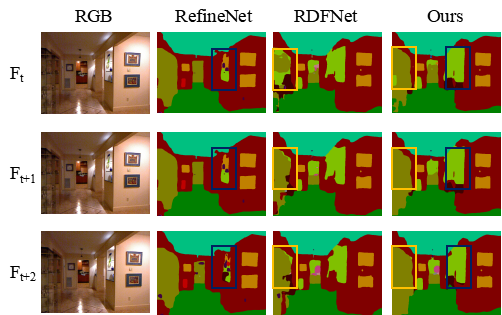
\includegraphics[scale=0.65]{figure/Consist.png}
	\vspace*{-0.6cm} 
	\caption{An illustration of jumping problem in video semantic segmentation. The predicted results of adjacent frames by different methods are shown. Our method generates more temporally consistent results, especially in the highlighted regions.}
	\label{fig:Consist}
	\vspace*{-0.35cm}
\end{figure}
}

Semantic segmentation is a fundamental part of scene understanding.
%
For indoor scenes, the cluttered backgrounds, large variety of scenes, object occlusions and various illumination pose a series of challenges for accurate semantic segmentation.
%
In recent years, a great deal of studies have been conducted for indoor scene semantic segmentation, and they can be mainly divided into three groups: semantic segmentation of a single RGB image, semantic segmentation of RGBD images, and multi-task learning methods.


\noindent \textbf{Semantic Segmentation of a Single Image.}
%
Fully convolutional network (FCN)~\cite{Long2015} is a pioneering work for pixel-wise segmentation. It first converts existing convolutional neural networks (CNN) constructed for classification for semantic segmentation.
%
To overcome the limitations of FCN that the network limited by a fixed-size receptive field, Noh \emph{et al.} \cite{Noh2015} proposed a novel deconvolution algorithm to segment finer object structures.
%
Bayesian SegNet~\cite{Kendall2015} performs visual scene understanding with a measure of model uncertainty to produce a probabilistic segmentation result.
%
To capture semantic correlations between neighboring patches and exploit patch-patch contextual information, Lin \emph{et al.}~\cite{Lin2016} formulated conditional random fields (CRFs) with CNN-based pairwise potential function. 
%
For generating fine prediction, a multi-path refinement network is proposed to effectively exploit multi-level features and refine the prediction step by step~\cite{Lin2017}.
%

\comments{
Semantic segmentation from a single image often leads to incomplete segmentation results. 
%
As the predictions from RefineNet \cite{Lin2017} shown in Fig.~\ref{fig:Consist}.
}

\begin{figure*}[htbp]
%	\vspace{-0.6cm}
	\setlength{\abovecaptionskip}{0pt} 
	\setlength{\belowcaptionskip}{10pt}
	\centering
	\centering
	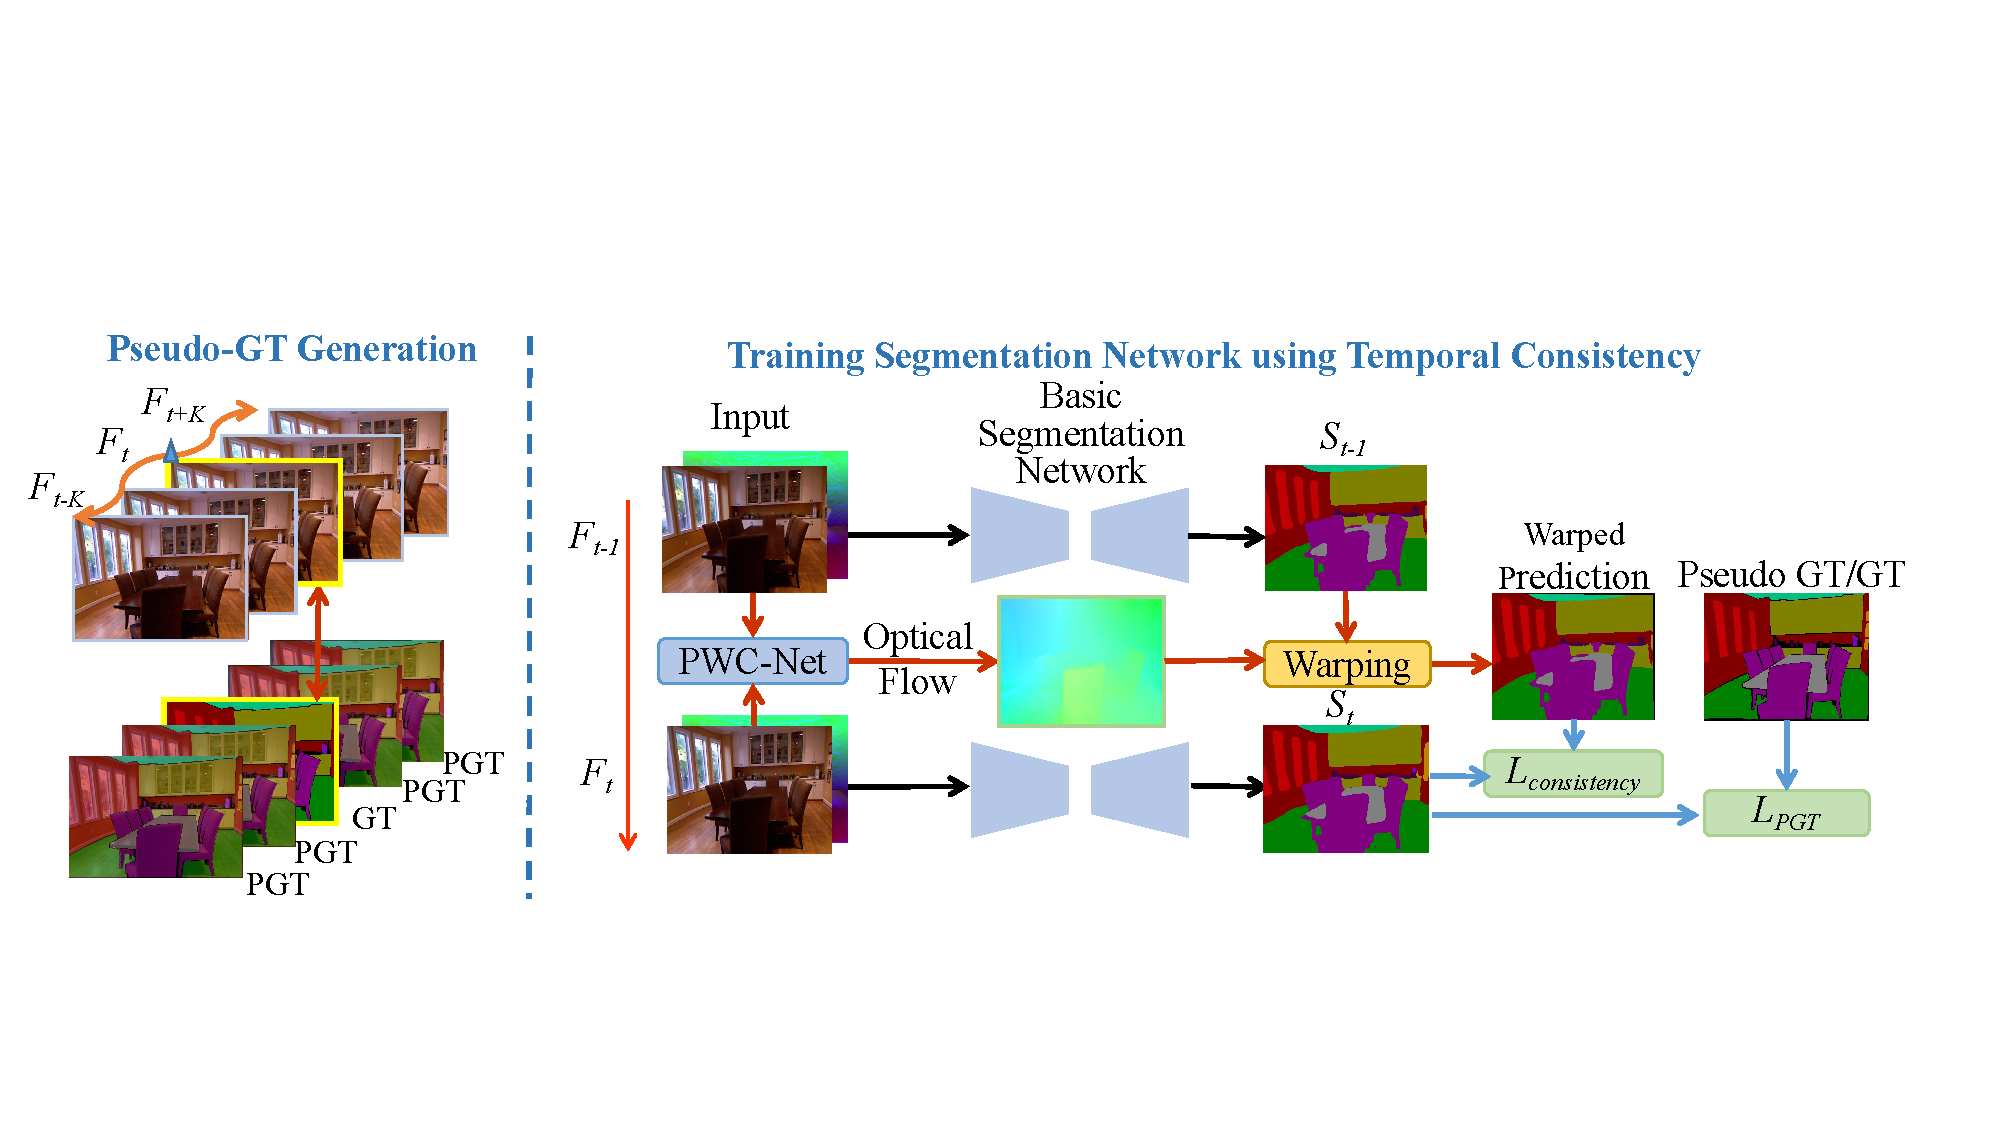
\includegraphics[scale=0.56]{figure/Pipeline.pdf}
%	\vspace*{-0.8cm} 
	\caption{The diagram of our proposed method. Left: we propagate the ground truth from a labeled frame to its adjacent frames by image warping. Right: the flowchart of our training strategy using temporal consistency. 
		%It mainly consists of three steps: 1) The current frame $F_t$ passes through a basic semantic segmentation network to generate the prediction  2) Warpping the prediction of previous frame $F_{t-1}$ depends on optical flow generated from PWC-Net \cite{Sun2018} 3) Warpped prediction of $F_{t-1}$ and generated PGT joint action on the network by $L_{consistency}$ and $L_{PGT}$ respectively.
		}
	\label{fig:Pipeline}
	\vspace*{-0.2cm}
\end{figure*}
 

\noindent \textbf{Semantic Segmentation of RGB-Depth Images.}
%
With the popularity of affordable depth-cameras, many techniques have been proposed for semantic segmentation of RGBD images.
%
Gupta \emph{et al.} \cite{Gupta2014} extracted features from RGB and depth data and integrated them for object detection and segmentation.
%
A novel long short-term memorized context fusion (LSTM-CF) model is proposed \cite{Li2016} to fuse contextual information from multiple sources such as RGB images and depth data.
% 
Cheng \emph{et al.} \cite{Cheng2017} rethink the relationship between RGB images and depth, and propose a locality-sensitive deconvolution network to refine object boundaries of segmentation result as well as a gated fusion layer to combine features of two modes.
%
Park \emph{et al.} \cite{Park2017} propose a multi-modal feature fusion blocks for fusing the multi-level RGB-D features and integrate these blocks into RefineNet.


 
\noindent \textbf{Multi-task Learning.} 
%
While semantic segmentation, depth estimation, and other tasks for indoor scene understanding share features, especially at shallow layers, many techniques have been proposed to train networks for multiple tasks in order to complement each other.
%
Eigen and Fergus \cite{Eigen2015} address three different tasks including depth prediction, surface normal estimation, and semantic labeling using a single multi-scale convolutional network. 
%
Prediction-and-distillationn network (PAD-Net)\cite{Xu2018} predicts a set of intermediate tasks including depth, surface normal, semantic and contour estimations, and then uses the predictions from these tasks as multi-modal distillation modules' inputs for final tasks.  
%
A novel joint Task-Recursive Learning (TRL) \cite{Zhang2018} framework for semantic segmentation and depth estimation is proposed by Zhang \emph{et al}. 
%
In TRL, two tasks are alternately processed in the decoder to improve each other.
% 
Jiao \emph{et al.} \cite{Jiao2018} present an attention-driven loss for network supervision and a synergy network to learn the information sharing strategies. 
%
By combining two tasks as well as proposed attention-driven loss, the performance of two tasks are mutually improved.
%
Although the multi-task learning methods improve the segmentation results, they require a lot of supplementary information or even dense-annotated data for other tasks.

Above approaches provide a lot of novel ideas to improve the segmentation results. However, the performance of these methods is greatly suppressed by limited densely annotated training data.
%
It is expensive and time-consuming to manually annotate semantic labels for images. 
%
In contrast, it is economical to capture videos, and the temporal correlation between adjacent frames naturally provides more information and constraints for the semantic labels. 
%
Therefore, we propose to improve existing networks for semantic segmentation by exploiting the temporal correlation between video frames in two aspects.
%In order to take full use of a large quantity of non-annotated data, in this paper, we propose two simple but effective approaches. 
%
First, instead of computing loss for each annotated image individually, we train a semantic segmentation network with a novel loss function to ensure the temporal consistency between adjacent frames in video sequences.
%
Second, with only a few labeled video frames, we propagate these labels to its neighboring frames with geometric transformations and generate a large number of new frames with pseudo ground truth (PGT) for network training. 
Compared to common data augmentation operations, it significantly increases the diversity of training data.
With these two training strategies, our approach achieves state-of-the-art performance on semantic segmentation for indoor scenes. 
%
\comments{
The rest of this paper is organized as follows.
% 
Our methodology will be introduced firstly.
%
Then, we will report the extensive experimental results as well as analyses. 
%
Finally we will draw a conclusion.}
